%% FullCourse_10Lecs -- Lecture 5, Topic 5.1: RL Framework, DP Connection, DP Limits
%% Source: ./archive_pre_split/Lec05_RL_Nutshell.tex (sections 1-3)
%% Pass B: compared against
%%         ../../MiniCourse_8hr/Slides/Module2_DL_RL_Macro/M2_T3_RL_Basics.tex
%% Result: FullCourse is a strict superset of MiniCourse content for T1.
%%   All MiniCourse frames (Why RL? slogan, MDP, MDP-meets-Growth, V/Q, Bellman,
%%   V-vs-Q comparison) are already present with equal or greater depth.
%% FullCourse-only frames (no MiniCourse counterpart):
%%   - Agent-Environment Interaction Loop (with diagram)
%%   - Theoretical Foundations of DP (Banach, Blackwell)
%%   - Full Expectation Backup --- DP's Core Computation
%%   - Curse of Dimensionality (Challenge 1)
%%   - Unknown or Intractable Environments (Challenge 2)
%%   - Why (Deep) Reinforcement Learning Helps
%%   - RL: Beyond Classical DP --- Summary
%%
%% Flow restructure (2026-07-08): one economist-first path through the act ---
%% "3 quiet requirements (R1 known model, R2 sweepable states, R3 no
%% exploration) -> 2 walls -> 3 departures (#1 sample the backup -> 5.2,
%% #2 approximate the function -> 5.3, #3 explore deliberately -> 5.2)".
%%   - NEW "This Act in Five Stops" frame (primary appendix entry point).
%%   - CUT "Why RL Exists" (content re-homed: credit assignment -> Common
%%     Pattern; Go hook -> Wall 1; opacity -> Wall 2; DQN/AlphaGo -> Why
%%     Deep RL Helps).
%%   - MERGED "From Static to Dynamic" + "RL in Economics" into one frame.
%%   - MOVED "V vs Q" from the DP section into the MDP section.
%%   - NEW "The Main Departures at a Glance" closer before the 2x2 map.
%% Net frame count unchanged: 24 main + 12 appendix.

%% Shared preamble for the FullCourse_10Lecs topic decks.
%%
%% Each topic .tex \input's this file, then defines its own \title, \date
%% override (if any), \graphicspath, and \begin{document}.
%%
%% Reconstructed verbatim from the inlined copy preserved in
%% Lec10_Case_Studies/Lec10_T8_Case6_DeepRamsey.tex (lines 23-190), which is
%% explicitly annotated there as "from ../shared_preamble.tex, copied verbatim".
%% Base preamble matches MiniCourse_8hr/Slides/shared_preamble.tex; this version
%% additionally provides \sectiondivider, the conceptbox/cautionbox/examplebox/
%% takeawaybox tcolorboxes, and \compacttables used across the split decks.

\documentclass[10pt,english,aspectratio=169]{beamer}

\usepackage{ae,aecompl}
\usepackage[T1]{fontenc}
\usepackage{textcomp}
\usepackage[utf8]{inputenc}
\usepackage{babel}
\usepackage{datetime2}

\setcounter{secnumdepth}{3}
\setcounter{tocdepth}{3}

\usepackage{amsmath, amssymb, amsthm, graphicx}
\usepackage{booktabs, multirow}
\usepackage{tikz}
\usepackage{pgfplots}
\pgfplotsset{compat=1.16}
\usepackage[most]{tcolorbox}
\tcbuselibrary{skins, breakable, theorems}
\usepackage{listings}
\usepackage{xcolor}

\lstset{
  basicstyle=\ttfamily\small,
  keywordstyle=\color{blue!80!black}\bfseries,
  commentstyle=\color{green!50!black}\itshape,
  stringstyle=\color{orange!80!black},
  backgroundcolor=\color{gray!8},
  frame=single,
  rulecolor=\color{gray!40},
  breaklines=true,
  showstringspaces=false,
  numbers=none,
}

\lstdefinestyle{pythonstyle}{
    language=Python,
    basicstyle=\ttfamily\footnotesize,
    keywordstyle=\color{blue!80!black}\bfseries,
    commentstyle=\color{green!50!black}\itshape,
    stringstyle=\color{orange!80!black},
    frame=single,
    breaklines=true,
    showstringspaces=false,
    numbers=left,
    numbersep=5pt,
    numberstyle=\tiny\color{gray},
    backgroundcolor=\color{gray!8},
    rulecolor=\color{gray!40}
}

\ifx\hypersetup\undefined
  \AtBeginDocument{%
    \hypersetup{bookmarks=false,breaklinks=true,pdfborder={0 0 0},colorlinks=true,
      linkcolor=DarkText,urlcolor=RedTitle}%
  }
\else
  \hypersetup{bookmarks=false,breaklinks=true,pdfborder={0 0 0},colorlinks=true,
    linkcolor=DarkText,urlcolor=RedTitle}%
\fi

\makeatletter
\newcommand\makebeamertitle{%
  \begin{frame}[plain]
    \vspace*{1.0cm}
    \centering
    {\usebeamerfont{title}\usebeamercolor[fg]{title}\inserttitle\par}
    \vspace{1.0cm}
    {\usebeamerfont{author}\usebeamercolor[fg]{author}\insertauthor\par}
    \vspace{0.2cm}
    {\usebeamerfont{date}\usebeamercolor[fg]{date}\insertdate\par}
  \end{frame}}%
\AtBeginDocument{%
  \let\origtableofcontents=\tableofcontents
  \def\tableofcontents{\@ifnextchar[{\origtableofcontents}{\gobbletableofcontents}}
  \def\gobbletableofcontents#1{\origtableofcontents}%
}

\usetheme{metropolis}
\usefonttheme{professionalfonts}

\definecolor{LightGray}{RGB}{230,230,230}
\definecolor{RedTitle}{RGB}{0,0,200}
\definecolor{VeryLightGray}{RGB}{245,245,245}
\definecolor{DarkText}{RGB}{0,0,0}

\setbeamercolor{background canvas}{bg=white}
\setbeamercolor{title}{fg=RedTitle}
\setbeamercolor{author}{fg=DarkText}
\setbeamercolor{date}{fg=DarkText}
\setbeamercolor{frametitle}{bg=VeryLightGray,fg=DarkText}
\setbeamercolor{normal text}{fg=DarkText}
\setbeamerfont{title}{size=\large}

\setbeamersize{text margin left=5mm, text margin right=5mm}
\addtobeamertemplate{frametitle}{}{\vspace{-0.5em}}
\newcommand{\reducevspace}{\vspace{-0.5cm}}

% Shared section divider and box styles for split topic decks.
\newcommand{\sectiondivider}[2]{%
\begin{frame}[plain,noframenumbering]
\begin{center}
\vfill
{\Large\textbf{#1}\par}
\vspace{0.35cm}
{\normalsize #2\par}
\vfill
\end{center}
\end{frame}
}

\newtcolorbox{conceptbox}[1][]{
  colback=blue!3,
  colframe=RedTitle!55,
  boxrule=0.35mm,
  arc=1mm,
  left=2mm,
  right=2mm,
  top=1mm,
  bottom=1mm,
  #1
}
\newtcolorbox{cautionbox}[1][]{
  colback=red!3,
  colframe=red!50!black,
  boxrule=0.35mm,
  arc=1mm,
  left=2mm,
  right=2mm,
  top=1mm,
  bottom=1mm,
  #1
}
\newtcolorbox{examplebox}[1][]{
  colback=green!3,
  colframe=green!45!black,
  boxrule=0.35mm,
  arc=1mm,
  left=2mm,
  right=2mm,
  top=1mm,
  bottom=1mm,
  #1
}
\newtcolorbox{takeawaybox}[1][]{
  colback=VeryLightGray,
  colframe=RedTitle!55,
  boxrule=0.35mm,
  arc=1mm,
  left=2mm,
  right=2mm,
  top=1mm,
  bottom=1mm,
  #1
}
\newcommand{\compacttables}{\renewcommand{\arraystretch}{1.15}}

\setbeamertemplate{navigation symbols}{}
\setbeamertemplate{footline}{%
  \hfill%
  \usebeamercolor[fg]{page number in head/foot}%
  \usebeamerfont{page number in head/foot}%
  \insertframenumber\,/\,\inserttotalframenumber\kern1em\vskip2pt%
}

\makeatother

\author{Zhigang Feng}
% "date with time": compile timestamp so each build is identifiable.
\date{\today\ \DTMcurrenttime}


% The undergrad-foundations appendix must not inflate the main deck's
% "k/Total" footer: restart frame numbering at \appendix.
\usepackage{appendixnumberbeamer}

\graphicspath{{./pic/}{../../MiniCourse_8hr/Slides/Module2_DL_RL_Macro/pic/}{../}}

% Suppress the redundant auto-generated metropolis section page; the
% \sectiondivider frames below are the dividers we keep.
\metroset{sectionpage=none}
\usetikzlibrary{positioning,arrows.meta,shapes,calc}
%% Lec05 shared MAP slide: "one backbone, three acts" recurring diagram.
%% Input this file AFTER ../shared_preamble.tex (needs RedTitle, VeryLightGray,
%% DarkText) and AFTER \usetikzlibrary{positioning,arrows.meta,shapes,calc}.
%% Call \LecFiveMap{k} inside a frame, where k in {1,2,3} highlights the current
%% act ("you are here") and k = 0 renders the closing reprise with all three
%% acts checked green (used by T3's closing synthesis frame).
%% Filename deliberately does NOT match the build glob Lec*_T*.tex, so the build
%% script never tries to compile it standalone.
%%
%% The three acts double as the lecture's spine: MODEL -> SAMPLE -> SCALE, i.e.
%% the three ways RL fills the Bellman expectation --- full backup (needs P,R),
%% sample backup (model-free), then sampled + function-approximated (deep RL).

\newcommand{\LecFiveMap}[1]{%
% Precompute per-box style selectors; TikZ option lists are comma-split before
% TeX conditionals run, so \ifnum must not sit inside a [...] options list.
\ifnum#1=0
  \tikzset{lmapa/.style={lmapdone}, lmapb/.style={lmapdone},
           lmapc/.style={lmapdone}}%
\else
  \tikzset{lmapa/.style={}, lmapb/.style={}, lmapc/.style={}}%
  \ifnum#1=1 \tikzset{lmapa/.style={lmapcur}}\fi
  \ifnum#1=2 \tikzset{lmapb/.style={lmapcur}}\fi
  \ifnum#1=3 \tikzset{lmapc/.style={lmapcur}}\fi
\fi
\begin{center}
\begin{tikzpicture}[
    act/.style={rectangle, rounded corners, draw=black!60, fill=VeryLightGray,
        minimum width=3.4cm, minimum height=1.0cm, text width=3.25cm,
        align=center, font=\small, text=DarkText},
    lmapcur/.style={draw=RedTitle, very thick, fill=orange!20},
    lmapdone/.style={draw=green!45!black, thick, fill=green!10},
    q/.style={font=\tiny\itshape, text width=3.4cm, align=center, text=black!70},
    barlab/.style={font=\tiny\bfseries, text=black!65},
    sat/.style={rectangle, rounded corners, draw=black!45, dashed, fill=white,
        text width=4.3cm, align=center, font=\tiny, text=black!70,
        minimum height=0.5cm},
    arr/.style={-{Stealth[length=2.4mm]}, thick, gray!60}
]
    % --- three act boxes ---
    \node[act, lmapa] (a1) at (0,0)
        {\textbf{5.1\ \ MODEL}\\[1pt] \tiny MDP \& the DP bridge};
    \node[act, lmapb] (a2) at (4.5,0)
        {\textbf{5.2\ \ SAMPLE}\\[1pt] \tiny MC $\cdot$ TD $\cdot$ Q-learning};
    \node[act, lmapc] (a3) at (9.0,0)
        {\textbf{5.3\ \ SCALE}\\[1pt] \tiny actor--critic $\cdot$ deep RL};
    \draw[arr] (a1) -- (a2);
    \draw[arr] (a2) -- (a3);
    % --- the student question each act answers ---
    \node[q] at (0,-0.98)   {what is RL, and how does it\\ relate to the DP I know?};
    \node[q] at (4.5,-0.98) {how do I learn a policy with\\ no model of the world?};
    \node[q] at (9.0,-0.98) {how does it scale --- and\\ where has it worked?};
    % --- "you are here" marker above the current act ---
    \ifnum#1=1 \node[font=\scriptsize\bfseries, text=RedTitle] at (0,1.02)
        {you are here\ $\blacktriangledown$};\fi
    \ifnum#1=2 \node[font=\scriptsize\bfseries, text=RedTitle] at (4.5,1.02)
        {you are here\ $\blacktriangledown$};\fi
    \ifnum#1=3 \node[font=\scriptsize\bfseries, text=RedTitle] at (9.0,1.02)
        {you are here\ $\blacktriangledown$};\fi
    \ifnum#1=0 \node[font=\scriptsize\bfseries, text=green!45!black] at (4.5,1.02)
        {all three acts complete};\fi
    % --- bottom band: the backup taxonomy (the technical spine of the lecture) ---
    \fill[blue!10]   (-1.6,-1.78) rectangle (1.6,-1.45);
    \fill[green!12]  (2.9,-1.78)  rectangle (6.1,-1.45);
    \fill[orange!16] (7.4,-1.78)  rectangle (10.6,-1.45);
    \node[barlab] at (0,-1.615)   {FULL BACKUP\ (needs $P,R$)};
    \node[barlab] at (4.5,-1.615) {SAMPLE BACKUP\ (model-free)};
    \node[barlab] at (9.0,-1.615) {SAMPLED $+$ APPROXIMATED};
    % --- dashed satellites: where this lecture sits in the course flow ---
    \node[sat] at (0,-2.45)
        {\textit{upstream:} Lec02 (RL = 3rd ML pillar), Lec04 T2 (RL as a Bellman solver)};
    \node[sat] at (9.0,-2.45)
        {\textit{downstream:} Lec06 --- HA models at scale (Aiyagari, Krusell--Smith, DeepHAM)};
\end{tikzpicture}
\end{center}
}


\title[AI for Econ Research]{AI for Economic Research: Dynamic Models, Language, and Agents\\
Lecture 5.1: The RL Framework and Its Link to Dynamic Programming}
\author{Zhigang Feng}
\date{\today\ \DTMcurrenttime}

\begin{document}

\makebeamertitle

%=============================================================================
\begin{frame}{Lecture 5 in One Map}
\textbf{One lecture, three decks, one idea: replace the model you must \emph{specify} with experience you can \emph{sample} --- then \emph{scale} it with function approximation.}

\LecFiveMap{1}

\vspace{0.05cm}
\footnotesize\textit{\textbf{Act 5.1 (here)} runs in five stops: what RL \emph{is} $\to$ your problem in MDP language $\to$ what classical DP quietly demands $\to$ where it breaks $\to$ the departures that become Acts 5.2--5.3. Running anchor throughout: the optimal growth model. New to dynamic macro? A self-contained appendix (Solow $\to$ Bellman) backs this deck --- the next slide says how to use it.}
\end{frame}

%=============================================================================
% NEW (flow restructure 2026-07-08): act-level path + prerequisite statement.
% This is the appendix's PRIMARY entry point --- announced before any DP
% machinery is used in anger, so newcomers learn the safety net exists
% before they need it. Point-of-need buttons remain on the growth-model,
% Bellman, and DP-foundations frames.
\begin{frame}{This Act in Five Stops --- and What It Assumes}
\begin{center}
\begin{tikzpicture}[
  pstep/.style={rectangle, rounded corners, draw=black!50, fill=VeryLightGray,
                minimum height=1.4cm, text width=2.15cm, align=center, inner sep=2pt},
  parr/.style={->, >=stealth, semithick, black!55}]
  \node[pstep] (p1) at (0,0)
    {\scriptsize\textbf{1\ \ What is RL?}\\[-1pt] \tiny act, observe reward, adjust};
  \node[pstep] (p2) at (2.8,0)
    {\scriptsize\textbf{2\ \ Your problem, their language}\\[-1pt] \tiny MDP $\leftrightarrow$ growth model};
  \node[pstep] (p3) at (5.6,0)
    {\scriptsize\textbf{3\ \ What DP demands}\\[-1pt] \tiny Bellman $+$ fine print};
  \node[pstep] (p4) at (8.4,0)
    {\scriptsize\textbf{4\ \ Where DP breaks}\\[-1pt] \tiny two walls};
  \node[pstep] (p5) at (11.2,0)
    {\scriptsize\textbf{5\ \ RL's departures}\\[-1pt] \tiny the plan for 5.2--5.3};
  \draw[parr] (p1) -- (p2); \draw[parr] (p2) -- (p3);
  \draw[parr] (p3) -- (p4); \draw[parr] (p4) -- (p5);
\end{tikzpicture}
\end{center}

\vspace{0.1cm}
\textbf{What the main track assumes:} you have met the \textbf{Bellman equation} and value function iteration (first-year macro). If that is you, this deck is self-contained --- stops 2--3 are home turf, revisited with RL eyes.

\vspace{0.15cm}
\begin{conceptbox}
\footnotesize\textbf{New to dynamic macro?} Appendix A1--A11 builds everything from the Solow model up --- self-contained, intuition first. \textbf{Minimum before stop 3:} A5 (the Bellman equation, read as one sentence) $+$ A8 (why iteration finds it). Best read in full after the session; buttons throughout the deck jump there and back.
\hfill\hyperlink{appFoundations}{\beamergotobutton{\scriptsize Appendix roadmap}}\normalsize
\end{conceptbox}
\end{frame}

%=============================================================================
% NEW: introductory "What is RL?" section --- intuition and examples before the formalism.
\section{What is Reinforcement Learning?}

\sectiondivider{What Is Reinforcement Learning?}{Intuition and everyday examples, before any formalism}

\begin{frame}{Reinforcement Learning: Learning by Trial and Error}
\begin{itemize}
  \item \textbf{Reinforcement learning (RL)}: an \textbf{agent} learns to make good decisions by \textbf{interacting} with an \textbf{environment} and observing a \textbf{reward}.
  \item No teacher hands it the right answer --- it learns from \textbf{consequences}: try, observe, adjust, repeat.
\end{itemize}
\vspace{0.2cm}
\begin{conceptbox}
\textbf{How RL differs from the other ML pillars:}
\begin{itemize}
  \item \textbf{Supervised} learning: data come with \textit{labels} (the correct answer).
  \item \textbf{Unsupervised} learning: find \textit{structure} in unlabeled data.
  \item \textbf{Reinforcement} learning: no labels --- only a \textit{scalar reward}, often \textit{delayed}, to be maximized over time.
\end{itemize}
\end{conceptbox}
\end{frame}

\begin{frame}{What Is RL? Three Everyday Examples}
\footnotesize
\begin{center}
\begin{tabular}{@{}p{2.7cm}p{2.8cm}p{2.8cm}p{2.8cm}@{}}
\toprule
\textbf{Setting} & \textbf{Action} & \textbf{Reward} & \textbf{What it learns} \\
\midrule
Playing a game \newline (Go, Atari, chess) & a move & win / lose, score & a winning \textbf{policy} \\
A child / robot \newline learning to walk & motor commands & progress; didn't fall & a stable \textbf{gait} \\
A/B testing \newline (web page, price) & which version to show & click / purchase & the best \textbf{option} \\
\bottomrule
\end{tabular}
\end{center}
\vspace{0.2cm}
\normalsize
\textbf{Common thread:} decisions are \textbf{sequential}, rewards can be \textbf{delayed}, and the agent must \textbf{explore} (try things) --- not just exploit what looks best so far.
\end{frame}

\begin{frame}{The Same Loop in Economics}
\begin{itemize}
  \item \textbf{Dynamic pricing:} a firm sets a \textit{price} (action), observes \textit{demand / profit} (reward), learns a \textbf{pricing rule}.
  \item \textbf{Monetary policy:} a central bank sets the \textit{interest rate} (action), observes \textit{inflation / output} (reward), learns a \textbf{policy rule}.
  \item \textbf{Consumption--savings:} a household chooses \textit{how much to save} (action), enjoys \textit{utility now} and carries \textit{wealth forward} (state), learns a \textbf{savings rule}.
\end{itemize}
\vspace{0.3cm}
\begin{takeawaybox}
These are exactly the \textbf{sequential decision problems} economists have long solved with \textbf{dynamic programming}. RL is a different way to attack the \emph{same} problems --- by learning from experience.
\end{takeawaybox}
\end{frame}

% MOVED here from the framework section: the agent--environment loop now introduces the common pattern.
\begin{frame}{The Common Pattern: Agent, Environment, Reward}
At each time step, the agent observes state $S_t$, chooses action $A_t$.
The environment returns reward $R_{t+1}$ and transitions to $S_{t+1}$.
\vfill
\centering
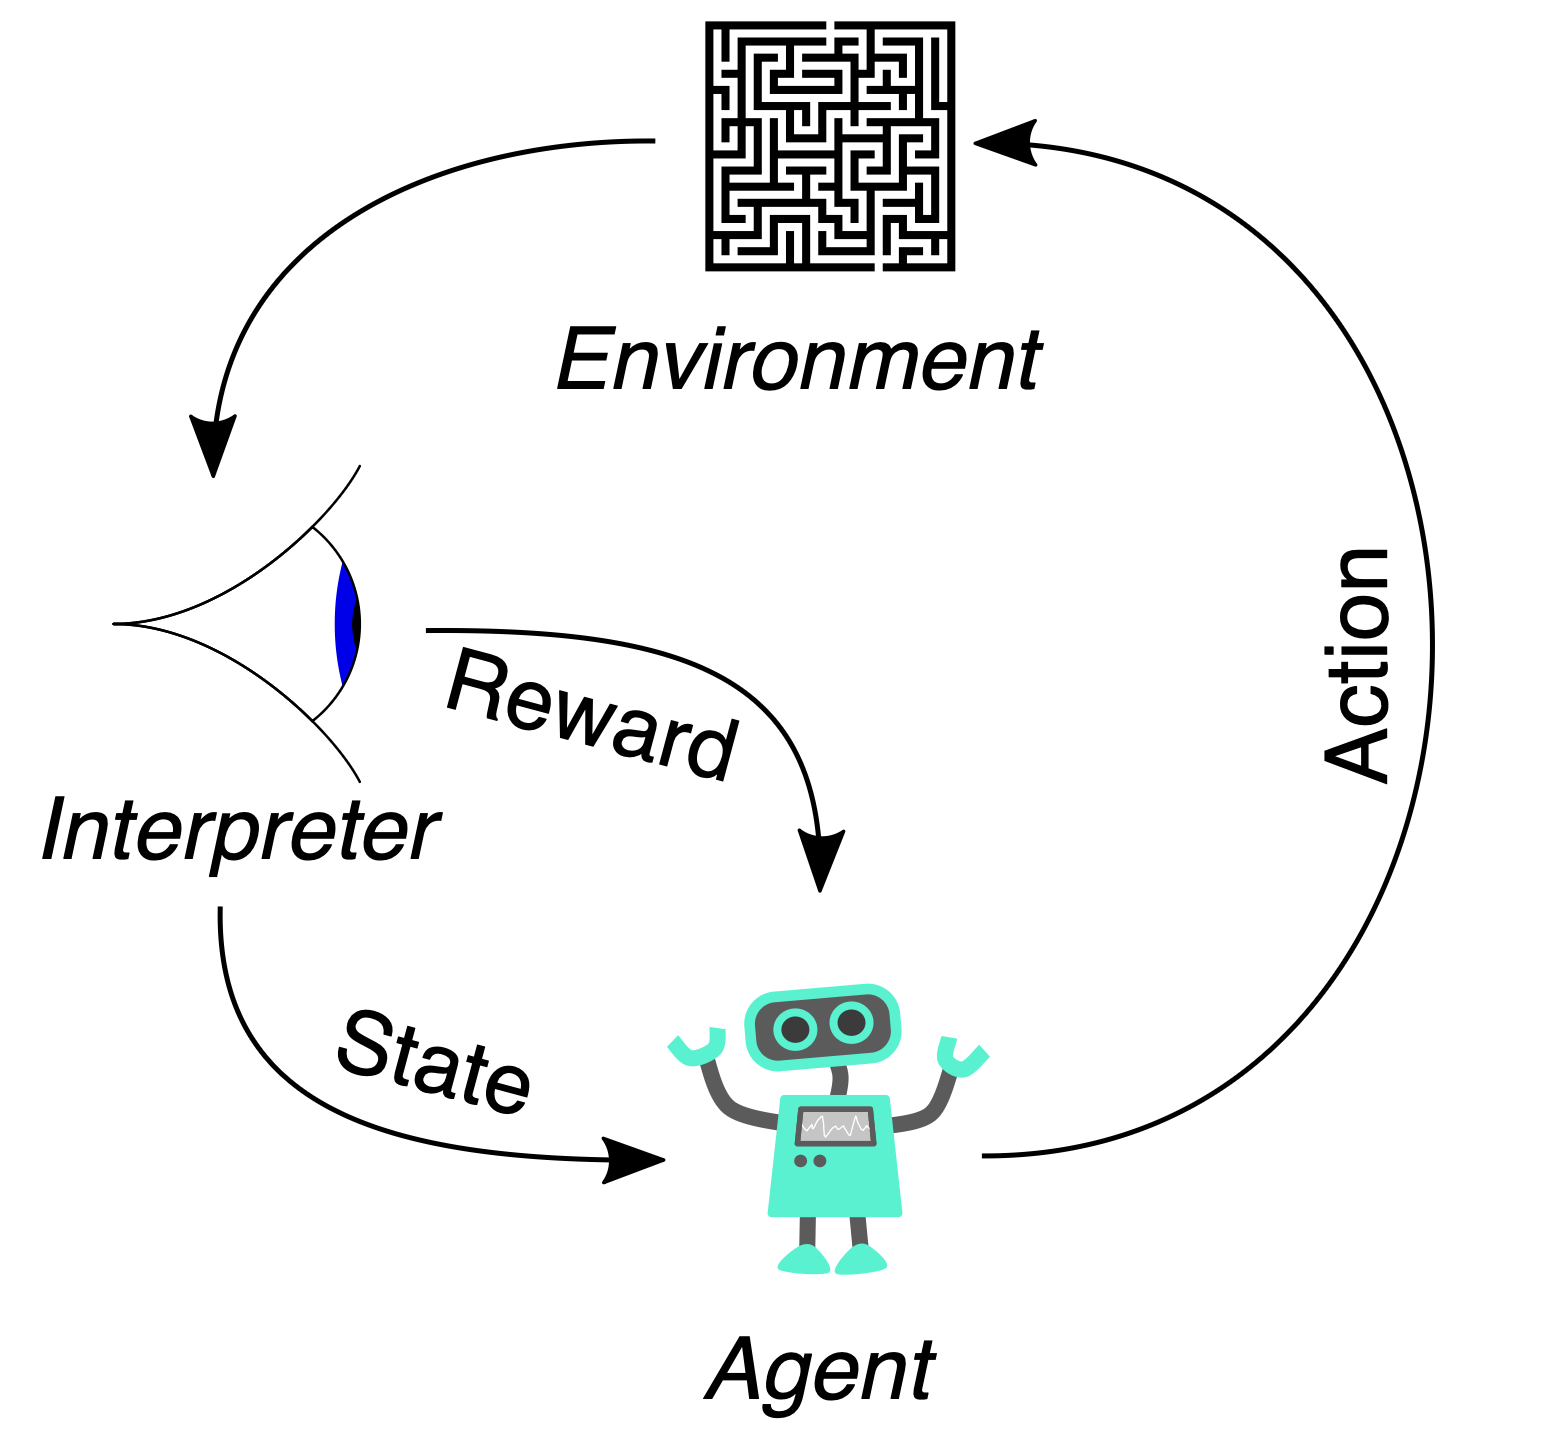
\includegraphics[width=4.8cm]{agent_env_loop.png}
\vfill
\small
\textbf{Trajectory:} $s_0, a_0, r_1, s_1, a_1, r_2, s_2, \ldots$
\quad The \textbf{return} (cumulative reward) from time $t$: $G_t = \sum_{k=0}^{\infty} \gamma^k r_{t+k+1}$.

\smallskip
\footnotesize
\textbf{The built-in difficulty:} rewards arrive \emph{late} --- which of the many past decisions earned them? This is the \textbf{credit-assignment problem} (Minsky); every algorithm in this lecture is, at heart, an answer to it.
\normalsize
\end{frame}

\begin{frame}{Two Ways to Solve a Dynamic Problem: Map vs.\ Explore}
\begin{columns}[T]
\column{0.48\textwidth}
\textbf{Dynamic Programming}\\\textit{``model first, then solve''}
\begin{itemize}
  \item Specify the environment fully ($P$, $R$).
  \item Compute $V$ at \textbf{every} state --- draw the complete map.
  \item Then act by the map.
  \item Like an \textbf{omniscient planner}.
\end{itemize}
\column{0.48\textwidth}
\textbf{Reinforcement Learning}\\\textit{``interact and learn''}
\begin{itemize}
  \item No complete map.
  \item \textbf{Walk} the environment repeatedly; update route judgments after each trip.
  \item Estimates approach what the map would say --- without ever drawing it.
  \item Like an \textbf{explorer}.
\end{itemize}
\end{columns}
\vspace{0.3cm}
\begin{conceptbox}
Same destination (the optimal policy), two routes. RL shines exactly when drawing the full map is \textbf{infeasible} --- \emph{when} and \emph{why} that happens is stops 3--4. First, we make both sides precise.
\end{conceptbox}
\end{frame}

% NOTE (2026-07-08): "Why RL Exists" frame cut; its content is re-homed where
% the logic needs it --- credit assignment -> "The Common Pattern" above; the
% Go scale hook -> Wall 1; opacity -> Wall 2; the DQN/AlphaGo takeoff note ->
% "Why (Deep) RL Helps".

%=============================================================================
\section{The MDP: Your Problem, Their Language}

\sectiondivider{The MDP: Your Problem, Their Language}{The formal RL toolkit --- and why it is the recursive problem economists already solve}

% MERGED (2026-07-08): "From Static to Dynamic: Why RL?" + "Reinforcement
% Learning in Economics" --- the two frames repeated Section 1's message.
\begin{frame}{Sequential Decision Problems: What We Are Formalizing}
\begin{itemize}
    \item The economic problems we formalize here are \textbf{sequential}:
    \begin{itemize}
        \item Consumption--saving \quad$\cdot$\quad firm investment and pricing \quad$\cdot$\quad monetary and fiscal policy.
    \end{itemize}
    \item Three features make them genuinely dynamic:
    \begin{enumerate}
        \item \textbf{Sequential}: decisions at every period, not once-and-for-all.
        \item \textbf{Intertemporal coupling}: today's consumption $\Rightarrow$ tomorrow's capital.
        \item \textbf{Uncertainty}: future shocks $z_{t+1}$ unknown at time $t$.
    \end{enumerate}
    \item The objective is \textbf{long-term} --- utility, profit, welfare --- so every choice must weigh its whole future.
    \item Economists solve this class with \textbf{dynamic programming}; RL formalizes the \emph{same} class as a \textbf{Markov decision process}. The dictionary between the two is next.
\end{itemize}
\end{frame}

\begin{frame}{Markov Decision Process (MDP) Formulation}
\begin{itemize}
  \item An RL problem is formalized as a \textbf{Markov Decision Process (MDP)}:
  \[
    \mathcal{M} = \langle \mathcal{S}, \mathcal{A}, P, R, \gamma \rangle.
  \]
  \item $\mathcal{S}$: set of \textbf{states} (e.g., capital $k$, shock $z$, wealth distribution $\Phi$).
  \item $\mathcal{A}$: set of \textbf{actions} (e.g., consumption $c$, investment $i$).
  \item $P: \mathcal{S}\times\mathcal{A} \to \Delta(\mathcal{S})$, $P(s'|s,a)$: \textbf{transition kernel}.
  \item $R: \mathcal{S}\times\mathcal{A} \to \mathbb{R}$, $R(s,a)$: \textbf{reward} (= instantaneous utility $u(c)$). \textit{Canonical form used throughout Lec05--Lec09.}
  \item $\gamma \in [0,1)$: \textbf{discount factor} ($= \beta$ in econ notation).
  \item \textbf{Objective:} Find an optimal policy $\pi^*$ that maximizes
  \[
    \mathbb{E}_\pi\!\left[\sum_{t=0}^\infty \gamma^t R(s_t, a_t)\right].
  \]
\end{itemize}
\end{frame}

\begin{frame}[label=mainWorkhorse]{MDP Meets the Growth Model}
\hfill\hyperlink{appFoundations}{\beamergotobutton{\scriptsize New to dynamic macro? Appendix: Solow $\to$ Bellman}}

\vspace{-0.15cm}
Consider the \textbf{optimal growth model}:
\[
\max_{\{c_t, k_{t+1}\}} \; \mathbb{E}_0 \sum_{t=0}^{\infty} \beta^t \, u(c_t)
\quad \text{s.t.} \quad
c_t + k_{t+1} = z_t f(k_t) + (1-\delta) k_t
\]

\vspace{0.2cm}
\begin{center}
\small
\begin{tabular}{ll}
\toprule
\textbf{MDP element} & \textbf{Growth model} \\
\midrule
State $s$ & $(k_t, z_t)$ --- capital + productivity \\
Action $a$ & $c_t$ (or equivalently $k_{t+1}$) \\
Transition $P(s'|s,a)$ & $k_{t+1} = (1-\delta)k_t + z_t f(k_t) - c_t$; $\log z_{t+1} = \rho \log z_t + \varepsilon_{t+1}$ \\
Reward $R(s,a)$ & $u(c_t)$ --- period utility \\
Discount $\gamma$ & $\beta$ --- household discount factor \\
Policy $\pi(s)$ & Consumption rule $c^*(k,z)$ \\
\bottomrule
\end{tabular}
\end{center}

\vspace{0.2cm}
The Bellman equation and MDP are two views of the \textbf{same} problem.
\end{frame}

% NOTE: "Agent--Environment Interaction Loop" moved to the intro section
% ("The Common Pattern: Agent, Environment, Reward").

\begin{frame}{Policy and Value Functions}
\begin{itemize}
    \item \textbf{Policy} $\pi$: a mapping from states to actions.
    \begin{itemize}
        \item Deterministic: $a = \pi(s)$ \quad (e.g., $c^*(k,z)$ in econ).
        \item Stochastic: $a \sim \pi(a|s)$ \quad (useful for exploration).
    \end{itemize}

    \vspace{0.3cm}
    \item \textbf{State-value function} --- expected return from state $s$ under $\pi$:
    \[
    V^\pi(s) = \mathbb{E}_\pi[G_t \mid s_t = s]
    = \mathbb{E}_\pi\!\left[\sum_{k=0}^{\infty} \gamma^k r_{t+k+1} \;\Big|\; s_t = s\right].
    \]

    \item \textbf{Action-value function} --- expected return for action $a$ in state $s$:
    \[
    Q^\pi(s,a) = \mathbb{E}_\pi[G_t \mid s_t = s, a_t = a].
    \]

    \item \textbf{Relationship:} $V^\pi(s) = \sum_{a} \pi(a|s)\, Q^\pi(s,a)$.
\end{itemize}
\end{frame}

% MOVED here (2026-07-08) from the DP section: this frame compares the two
% cultures' emphases on V vs Q --- framework material, and its closing line
% previews Wall 2 (unknown environments).
\begin{frame}{$V(s)$ vs.\ $Q(s,a)$: Economics vs.\ Engineering}
\begin{columns}
\column{0.48\textwidth}
\textbf{Economics: Focus on $V(s)$}
\begin{itemize}
    \item Emphasis on \textbf{welfare/utility} from a given state.
    \item Optimal policies derived from planner's problem or equilibrium.
    \item DP solves for $V^\pi(s)$ directly.
    \item Rational agents optimize implicitly.
\end{itemize}

\column{0.48\textwidth}
\textbf{RL / Engineering: Focus on $Q(s,a)$}
\begin{itemize}
    \item Emphasis on \textbf{real-time action selection}.
    \item Learning $Q(s,a)$ allows decision-making \textbf{without a model}.
    \item $\pi^*(s) = \arg\max_a Q^*(s,a)$.
    \item Works in unknown environments.
\end{itemize}
\end{columns}

\vspace{0.5cm}
\textbf{Growing convergence:} As economists tackle complex, partially-known environments (heterogeneous agents, financial markets), the Q-function approach becomes increasingly valuable.
\end{frame}


%=============================================================================
\section{The Bellman Connection --- and What DP Demands}

\sectiondivider{The Bellman Connection}{Economists' old friend is RL's backbone --- plus the fine print classical DP relies on}

% NEW (Part-1 framing): why the structural tradition specifies, then solves.
\begin{frame}{Why Economists Specify, Then Solve}
\begin{itemize}
  \item Economists \textbf{write the model down first} --- preferences $u(\cdot)$, technology $f(k)$, constraints, shock process --- \emph{then} solve it.
  \item \textbf{Why?} Each primitive carries economic meaning ($\beta$ patience, $\alpha$ factor share, $\delta$ depreciation), so the solution inherits:
  \begin{itemize}
    \item \textbf{Interpretability} --- parameters are economic magnitudes.
    \item \textbf{Welfare analysis} --- integrate the same $u(c)$ that defines behavior.
    \item \textbf{Equilibrium-consistent prices} --- $r = z f'(k)-\delta$, $w = z[f(k)-kf'(k)]$ are \textit{competitive factor prices}, not reduced-form fits.
  \end{itemize}
  \item Disciplined by the \textbf{Lucas critique}: decision rules \emph{shift} when policy shifts, so a rule fit to historical behavior can fail once deployed --- better to solve a \textbf{structural} model.
\end{itemize}
\end{frame}

\begin{frame}{The Bellman Equation --- Economists' Old Friend}
\hfill\hyperlink{appBellman}{\beamergotobutton{\scriptsize Gentler build-up: Appendix A5}}

\vspace{-0.15cm}
\begin{itemize}
    \item Economists compute the value function $V(s)$ via the Bellman equation:
    \[
        V(s) = \max_{a}\Bigl\{ R(s,a) + \gamma \,\mathbb{E}[V(s') \mid s,a] \Bigr\}.
    \]
    \item Define the \textbf{Bellman operator} $T$:
    \[
    (TV)(s) = \max_{a} \left\{ R(s,a) + \gamma \sum_{s'} P(s'|s,a)\, V(s') \right\}.
    \]
    \item The value function is the \textbf{fixed point}: $V^* = TV^*$.
\end{itemize}
\end{frame}

% FullCourse-only: Banach contraction + Blackwell sufficient conditions
\begin{frame}[label=mainVFI]{Theoretical Foundations of DP}
\hfill\hyperlink{appCMT}{\beamergotobutton{\scriptsize Why these hold: Appendix A8--A9}}

\vspace{-0.15cm}
Three pillars guarantee that DP ``works'':

\begin{enumerate}
    \item \textbf{Principle of Optimality} (Bellman):
    \begin{itemize}
        \item Any tail of an optimal plan is itself optimal from the state it reaches.
        \item Guarantees \textbf{equivalence} between the sequence problem and the recursive formulation.
    \end{itemize}

    \item \textbf{Contraction Mapping Theorem} (Banach fixed-point theorem):
    \begin{itemize}
        \item $\|TV_1 - TV_2\|_\infty \leq \gamma \|V_1 - V_2\|_\infty$ for any $V_1, V_2$.
        \item Guarantees \textbf{existence}, \textbf{uniqueness}, and \textbf{convergence} of VFI.
    \end{itemize}

    \item \textbf{Blackwell's Sufficient Conditions} \hfill\footnotesize{Blackwell (1965), \emph{Ann.\ Math.\ Stat.}}\normalsize:
    \begin{itemize}
        \item \textbf{Monotonicity:} $V_1 \leq V_2 \Rightarrow TV_1 \leq TV_2$.
        \item \textbf{Discounting:} $T(V+c) \leq TV + \gamma c$ for $c \geq 0$.
        \item Easy-to-check conditions that imply contraction.
    \end{itemize}
\end{enumerate}
\vspace{0.15cm}
\footnotesize\textit{Economists \textbf{prize uniqueness}: it makes ``the model predicts $X$'' well-posed --- no ambiguity over which solution to report, which is what lends structural counterfactuals their credibility.}\normalsize
\end{frame}

% FullCourse-only, REWORKED (2026-07-08): full-expectation-backup formula plus
% the three-requirement checklist (R1/R2/R3) that the next section knocks down
% wall by wall --- the hinge of the whole act.
\begin{frame}{Full Expectation Backup --- and DP's Quiet Requirements}
The heart of Value Function Iteration (VFI):
\vspace{-0.1cm}
\[
(TV)(k,z) = \max_{k'} \left\{ u(c) + \beta \sum_{z' \in \mathcal{Z}} P(z'|z) \, V(k',z') \right\}
\]
\vspace{-0.35cm}

\small a \textbf{full expectation backup}: to update $V$ at \emph{one} state, sum over \textbf{all} possible next states, weighted by their probabilities.\normalsize

\vspace{0.05cm}
\textbf{The fine print --- three requirements so routine we forget they are assumptions:}
\footnotesize
\begin{enumerate}
    \item[\textbf{R1}] \textbf{A known model:} the law of motion and $P(z'|z)$ must be \emph{writable} --- else nothing to sum over.
    \item[\textbf{R2}] \textbf{A sweepable state space:} $V$ is a table on a grid, updated state by state --- feasible only if the states can be enumerated.
    \item[\textbf{R3}] \textbf{No exploration needed:} with the model in hand, the $\max$ \emph{inspects} every action's consequence --- nothing is ever tried.
\end{enumerate}
\normalsize
\vspace{0.05cm}
\begin{tcolorbox}[colback=VeryLightGray,colframe=RedTitle!60]
\footnotesize Each requirement fails somewhere economically important. The next stop shows where --- and each failure gets its own RL fix.\normalsize
\end{tcolorbox}
\end{frame}


%=============================================================================
% FullCourse-only section (retitled 2026-07-08): the two walls, then the
% three departures --- the act's payoff and the plan for Acts 5.2/5.3.
\section{Where DP Breaks --- and How RL Answers}

\sectiondivider{Where DP Breaks --- and How RL Answers}{Two walls, three departures --- the plan for the rest of the lecture}

\begin{frame}{Wall 1: The Curse of Dimensionality --- R2 Falls}
\textbf{The wall is not exotic.} Go's rules fit on one page, yet the game has $\approx 10^{170}$ legal positions (vs.\ $\sim 10^{80}$ atoms in the universe) --- a \emph{fully known} model, and still no table, no enumeration, no sweep.

\vspace{0.15cm}
\textbf{Economics hits the same wall sooner:}
\begin{itemize}
    \item VFI requires a \textbf{grid} over the state space. 2D model $(k, z)$: $100 \times 100 = 10{,}000$ points --- easy.
    \item Multi-sector model with $d$ state variables, $m$ grid points each: $m^d$ points.
    \begin{itemize}
        \item $d = 5,\; m = 100$: $10^{10}$ points. \quad $d = 8,\; m = 100$: $10^{16}$ points --- \textbf{completely infeasible}.
    \end{itemize}
    \item Sparse grids (Smolyak) and projection methods (Chebyshev) partially mitigate this, but break down beyond $\sim$5--8 dimensions.
    \item \textbf{Heterogeneous agents} make it worse: the wealth \textbf{distribution} $\Phi$ is itself a state variable --- an infinite-dimensional object. Krusell--Smith (1998) approximates $\Phi$ by its mean $K$, but accuracy degrades in complex models.
\end{itemize}
\end{frame}

\begin{frame}{Wall 2: Unknown or Intractable Environments --- R1 Falls}
\textbf{Some environments cannot be written down --- only interacted with:} robot dynamics, city traffic, a strategic opponent. Engineering built RL for exactly this. Economics has its own version:
\begin{itemize}
    \item In a representative-agent model: agent knows own state $\Rightarrow$ knows prices $\Rightarrow$ environment is \textbf{transparent}.
    \item In a heterogeneous-agent model:
    \begin{itemize}
        \item Prices depend on aggregate capital $K = \int a\, d\Phi(a,z)$.
        \item Individual agent does \textbf{not observe} $\Phi$ directly.
        \item The distribution's law of motion $\Phi' = \mathcal{T}(\Phi)$ has no closed form in general.
    \end{itemize}
    \item The ``environment'' (price dynamics) that an agent faces is \textbf{endogenous} and \textbf{unknown}.
\end{itemize}

\vspace{0.15cm}
\begin{tcolorbox}[colback=VeryLightGray,colframe=RedTitle!60]
\textbf{The core issue for economists:} prices \emph{are} the environment. When prices depend on distributions you cannot track, the environment becomes something you must \textit{learn} rather than \textit{specify}.
\end{tcolorbox}
\end{frame}


\begin{frame}{Why (Deep) Reinforcement Learning Helps}
\begin{enumerate}
    \item \textbf{Flexible Function Approximation (Neural Networks):}
    \begin{itemize}
        \item Traditional DP uses structured grids (Chebyshev, splines) that scale exponentially.
        \item Neural networks approximate $V(s)$ or $\pi(s)$ \textbf{without a grid}; parameters scale gracefully with dimension.
    \end{itemize}

    \vspace{0.2cm}
    \item \textbf{Sample-Based Learning (No Full Expectation Backup):}
    \begin{itemize}
        \item RL uses \textbf{simulated trajectories} instead of summing over all $s'$.
        \item Targets \textbf{relevant regions} of the state space via experience.
        \item Especially valuable when $\Phi$'s law of motion lacks a closed form.
    \end{itemize}

    \vspace{0.2cm}
    \item \textbf{Hardware Acceleration (GPUs/TPUs):}
    \begin{itemize}
        \item NN training = large-scale matrix multiplication $\Rightarrow$ GPU-friendly.
        \item Traditional grid-based DP does not map as naturally onto GPU architectures.
    \end{itemize}
\end{enumerate}

\vspace{0.1cm}
\begin{takeawaybox}
\footnotesize The ideas are old; the takeoff is recent. Core RL dates to the 1980s--90s, but it only ``\textbf{flew}'' once \textbf{deep learning} supplied efficient \textbf{function approximation in high dimensions}: \textbf{DQN} (Atari from raw pixels, 2015) and \textbf{AlphaGo} (2016). We return to AlphaGo in T3.\normalsize
\end{takeawaybox}
\end{frame}

%=============================================================================
% NEW (2026-07-08): the act's punchline --- every broken requirement mapped to
% its RL departure and to the act that delivers it. This is the overview frame
% the deck lacked: problem side (unknown env, high dim) x method side
% (sampling, deep-NN approximation, exploration).
\begin{frame}{The Main Departures at a Glance}
\textbf{Same Bellman backbone --- three departures from classical DP:}
\vspace{0.15cm}
\footnotesize
\begin{center}
\begin{tabular}{@{}p{2.9cm}p{2.9cm}p{4.3cm}p{1.4cm}@{}}
\toprule
\textbf{Classical DP pillar} & \textbf{The wall} & \textbf{RL's departure} & \textbf{Where} \\
\midrule
Full expectation backup --- needs $P$, $R$ \ (R1) & environment unknown or endogenous & \textbf{\#1 Sample the backup:} learn from trajectories --- Monte Carlo, TD, Q-learning & Act 5.2 \\
\addlinespace[3pt]
Value stored in a table / on a grid \ (R2) & curse of dimensionality & \textbf{\#2 Approximate the function:} neural $V$, $Q$, $\pi$ --- DQN, actor--critic & Act 5.3 \\
\addlinespace[3pt]
The $\max$ inspects every action \ (R3) & samples only show what you \emph{try} & \textbf{\#3 Explore deliberately:} $\epsilon$-greedy, Boltzmann, UCB --- the price of \#1 & Act 5.2 \\
\bottomrule
\end{tabular}
\end{center}
\normalsize
\vspace{0.15cm}
\begin{takeawaybox}
\textbf{The whole lecture in one sentence:} the Bellman backbone never changes --- only \emph{how the expectation is filled}: full backup (5.1) $\to$ sample backup (5.2) $\to$ sampled $+$ approximated (5.3).
\end{takeawaybox}
\end{frame}


% NEW (Part-3 preview): when DP vs when RL, and the structural special-case relationship.
\begin{frame}{When DP, When RL? A $2\times2$ Map}
\small
\begin{center}
\begin{tabular}{@{}p{2.0cm}p{5.4cm}p{5.4cm}@{}}
\toprule
 & \textbf{Model known} ($P$ available) & \textbf{Model unknown / intractable} \\
\midrule
\textbf{Low-dim} & Textbook DP (VFI / PI) --- \textit{RL buys little} & Tabular RL (Q-learning, SARSA) \\
\textbf{High-dim} & ``Deep DP'': NN approximation \emph{inside} VFI & Deep RL's home turf (HA models, market design) \\
\bottomrule
\end{tabular}
\end{center}
\vspace{0.25cm}
\normalsize
\begin{conceptbox}
\textbf{DP is RL's \emph{structural} special case:} when $P$ is known and $|\mathcal{S}|$ is small, sample backup $\to$ full backup and function approximation $\to$ table. (A statement about the \emph{equations}, not a free convergence guarantee.) So RL \textbf{extends} DP --- it does not replace it. And RL is \emph{not merely a last resort}: even with $P$ known, sampling $+$ approximation can win in high dimensions.
\end{conceptbox}
\end{frame}

\begin{frame}{RL: Beyond Classical DP --- Summary}
    \begin{itemize}
        \item RL algorithms (Q-learning, SARSA, actor-critic) extend DP to:
        \begin{itemize}
            \item Handle \textbf{unknown} transition models (model-free).
            \item Address \textbf{exploration--exploitation} directly.
            \item \textbf{Scale up} through function approximation.
        \end{itemize}
        \item Two pathways:
        \begin{itemize}
            \item \textbf{Model-free RL:} learn policies purely from observed data without explicit transition models.
            \item \textbf{Model-based RL:} combine simulation from approximate structural models with learning.
        \end{itemize}
    \end{itemize}

    \vspace{0.2cm}
    \begin{takeawaybox}
    \footnotesize The two RL pathways differ only in \emph{where the samples come from} --- a real/observed environment (model-free) or a simulated structural model (model-based). Either way, the Bellman backbone is unchanged; only the \emph{backup} changes.
    \end{takeawaybox}
\end{frame}

%=============================================================================
% House-style bridge closer (matches Lec09): restate the act, hand off to T2.
\begin{frame}{Bridge: From a Model You \emph{Specify} to Experience You \emph{Sample}}
\textbf{Act 5.1 framed the problem. Every sequential economic decision is an MDP; the Bellman equation economists already use \emph{is} RL's backbone; and classical DP's three quiet requirements --- a known model (R1), a sweepable state space (R2), no need to explore (R3) --- each fail somewhere economics cares about.}

\vspace{0.2cm}
\begin{itemize}
  \item That leaves three departures on the table: \textbf{\#1 sample the backup}, \textbf{\#2 approximate the function}, \textbf{\#3 explore deliberately}.
  \item \textbf{Next (5.2) executes \#1 --- and pays its price, \#3.} The question changes from ``how do we \emph{specify} the model?'' to ``how do we \emph{learn a good policy without one?}'' --- Monte Carlo, temporal-difference, and Q-learning replace the full expectation backup with a \textbf{sample} backup. Act 5.3 then delivers \#2 at scale.
  \item \footnotesize\textit{If the DP side moved fast: Appendix A1--A11 rebuilds it from Solow, self-contained --- T2 needs only the Bellman equation and the full-vs-sample backup distinction.}\normalsize
\end{itemize}

\vspace{0.1cm}
\begin{center}
\footnotesize\textit{Arc: \textbf{5.1 MODEL} (framework $+$ DP) $\;\to\;$ 5.2 SAMPLE (MC / TD / Q-learning) $\;\to\;$ 5.3 SCALE (actor--critic $+$ deep RL $+$ applications).}
\end{center}
\end{frame}

%=============================================================================
%  APPENDIX --- Dynamic Macro Foundations (undergraduate refresher)
%  Self-contained build-up from the Solow model to the recursive toolkit,
%  for audiences meeting dynamic macro for the first time. Embedded from
%  Lec04_T1_Motivation_Growth.tex (2026-07-08), cross-references retargeted
%  to this deck. Entry buttons sit on the "MDP Meets the Growth Model" frame
%  (label mainWorkhorse) and the "Theoretical Foundations of DP" frame
%  (label mainVFI); every appendix frame returns to the former.
%=============================================================================
\appendix
% Metropolis's \appendix hook swaps back its own plain footline with
% numbering=none, silently erasing the shared-preamble "k/Total" footer.
% Re-assert the house footline so appendix pages number as 1/12 ... 12/12
% (appendix-local, courtesy of appendixnumberbeamer).
\setbeamertemplate{footline}{%
  \hfill%
  \usebeamercolor[fg]{page number in head/foot}%
  \usebeamerfont{page number in head/foot}%
  \insertframenumber\,/\,\inserttotalframenumber\kern1em\vskip2pt%
}

\sectiondivider{Appendix: Dynamic Macro Foundations}{From Solow to Bellman --- a self-contained refresher, no dynamic macro assumed\\ (statements and intuition only; proofs live in your macro-theory course)}

%---------------------------------------
\begin{frame}[label=appFoundations]{Appendix Roadmap: From Solow to Bellman}
\textit{\footnotesize Everything the lecture takes for granted, built in eleven short steps --- click any step to jump; the arrow button on every page returns to the lecture.}
\hfill\hyperlink{mainWorkhorse}{\beamerreturnbutton{\scriptsize Return to lecture}}

\vspace{0.05cm}
\begin{center}
\begin{tikzpicture}[
  astep/.style={rectangle, rounded corners, draw=black!50, fill=VeryLightGray,
               minimum width=3.0cm, text width=2.9cm, minimum height=0.74cm,
               align=center, inner sep=2pt},
  grp/.style={font=\tiny\bfseries, text=RedTitle, anchor=west},
  arr/.style={->, >=stealth, semithick, black!55}]
  % --- Row 1: build the model ---
  \node[grp] at (-1.5,2.62) {BUILD THE MODEL};
  \node[astep] (s1) at (0,1.9)
    {\scriptsize\hyperlink{appSolow}{\textbf{A1\ \ Solow}}\\[-1pt] \tiny growth without choices};
  \node[astep] (s2) at (3.6,1.9)
    {\scriptsize\hyperlink{appRamsey}{\textbf{A2\ \ Add preferences}}\\[-1pt] \tiny saving becomes a choice};
  \node[astep] (s3) at (7.2,1.9)
    {\scriptsize\hyperlink{appSeqProblem}{\textbf{A3\ \ Sequential problem}}\\[-1pt] \tiny choose an infinite path};
  \node[astep] (s4) at (10.8,1.9)
    {\scriptsize\hyperlink{appMarkov}{\textbf{A4\ \ Markov structure}}\\[-1pt] \tiny the state $(k,z)$};
  \draw[arr] (s1) -- (s2); \draw[arr] (s2) -- (s3); \draw[arr] (s3) -- (s4);
  % --- Row 2: two formulations, one problem ---
  \node[grp] at (-1.5,0.72) {TWO FORMULATIONS, ONE PROBLEM};
  \node[astep] (s5) at (0,0)
    {\scriptsize\hyperlink{appBellman}{\textbf{A5\ \ Bellman equation}}\\[-1pt] \tiny recursion $+$ intuition};
  \node[astep] (s6) at (3.6,0)
    {\scriptsize\hyperlink{appEquivalence}{\textbf{A6\ \ Equivalence}}\\[-1pt] \tiny the four questions};
  \node[astep] (s7) at (7.2,0)
    {\scriptsize\hyperlink{appFunction}{\textbf{A7\ \ One function}}\\[-1pt] \tiny ``finite''-dimensional};
  \draw[arr, rounded corners=3pt] (s4.south) -- (10.8,0.95) -- (0,0.95) -- (s5.north);
  \draw[arr] (s5) -- (s6); \draw[arr] (s6) -- (s7);
  % --- Row 3: why it all works ---
  \node[grp] at (-1.5,-1.18) {WHY IT ALL WORKS};
  \node[astep] (s8) at (0,-1.9)
    {\scriptsize\hyperlink{appCMT}{\textbf{A8\ \ Contraction}}\\[-1pt] \tiny VFI must converge};
  \node[astep] (s9) at (3.6,-1.9)
    {\scriptsize\hyperlink{appBlackwell}{\textbf{A9\ \ Blackwell}}\\[-1pt] \tiny two easy conditions};
  \node[astep] (s10) at (7.2,-1.9)
    {\scriptsize\hyperlink{appBerge}{\textbf{A10\ \ Nice properties}}\\[-1pt] \tiny continuity, concavity};
  \node[astep] (s11) at (10.8,-1.9)
    {\scriptsize\hyperlink{appSummary}{\textbf{A11\ \ Summary}}\\[-1pt] \tiny $+$ where to learn more};
  \draw[arr, rounded corners=3pt] (s7.south) -- (7.2,-0.95) -- (0,-0.95) -- (s8.north);
  \draw[arr] (s8) -- (s9); \draw[arr] (s9) -- (s10); \draw[arr] (s10) -- (s11);
\end{tikzpicture}
\end{center}
\end{frame}

%---------------------------------------
\begin{frame}[label=appSolow]{Appendix A1 --- Where It All Starts: The Solow Growth Model}
\textit{\footnotesize The one dynamic model every undergraduate meets --- capital accumulation with a rule-of-thumb saver.}
\hfill\hyperlink{mainWorkhorse}{\beamerreturnbutton{\scriptsize Return to lecture}}

\vspace{0.1cm}
\begin{columns}
  \begin{column}{0.56\textwidth}
    \footnotesize
    \textbf{Technology} (per-worker terms): output from capital,
    $y_t = f(k_t) = A k_t^{\alpha}$, $\alpha\in(0,1)$ (diminishing returns).

    \smallskip
    \textbf{Behavior --- one assumed number}: save a \emph{fixed} fraction $s$ of output: $i_t = s\,y_t$, consume the rest, $c_t=(1-s)\,y_t$.

    \smallskip
    \textbf{The engine} --- capital accumulation:
    \[ k_{t+1} = (1-\delta)\,k_t + s A k_t^{\alpha} \]

    \textbf{Steady state} (saving $=$ replacement):
    $\;sAk^{*\alpha} = \delta k^{*} \Rightarrow k^{*} = \left(sA/\delta\right)^{\frac{1}{1-\alpha}}$; concavity makes it unique, with monotone convergence from any $k_0>0$.
  \end{column}
  \begin{column}{0.44\textwidth}
    \centering
    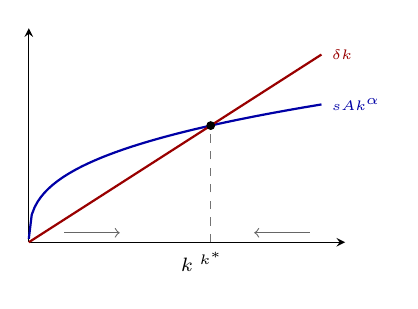
\begin{tikzpicture}
    \begin{axis}[width=5.6cm, height=4.3cm,
      axis lines=left, xlabel={\scriptsize $k$},
      xtick=\empty, ytick=\empty, xmin=0, xmax=4.0, ymin=0, ymax=1.35,
      clip=false, every axis plot/.append style={thick}]
      \addplot[domain=0.0001:3.7, samples=100, blue!65!black] {0.55*x^0.35}
        node[pos=1, right, font=\tiny, text=blue!65!black] {$sAk^{\alpha}$};
      \addplot[domain=0:3.7, red!60!black] {0.32*x}
        node[pos=1, right, font=\tiny, text=red!60!black] {$\delta k$};
      \draw[dashed, black!55] (axis cs:2.30,0) -- (axis cs:2.30,0.736);
      \fill (axis cs:2.30,0.736) circle[radius=1.6pt];
      \node[below, font=\tiny] at (axis cs:2.30,0) {$k^{*}$};
      \draw[->, black!60] (axis cs:0.45,0.06) -- (axis cs:1.15,0.06);
      \draw[->, black!60] (axis cs:3.55,0.06) -- (axis cs:2.85,0.06);
    \end{axis}
    \end{tikzpicture}

    \vspace{0.02cm}
    \tiny\textit{Below $k^{*}$ saving exceeds replacement, so $k$ grows; above, it shrinks --- the arrows on the axis.}
  \end{column}
\end{columns}
\vspace{0.05cm}
\begin{takeawaybox}
\footnotesize \textbf{Growth without choices.} Given $s$, the dynamics are fully mechanical --- nobody in the model ever decides anything. Solow (1956, \emph{QJE}) explains capital accumulation but stays silent on welfare: is $s$ a \emph{good} saving rate?
\end{takeawaybox}
\end{frame}

%---------------------------------------
\begin{frame}[label=appRamsey]{Appendix A2 --- From Solow to Optimal Growth: Make Saving a Choice}
\textit{\footnotesize Same technology, new question: instead of assuming how much society saves, derive it from preferences.}
\hfill\hyperlink{mainWorkhorse}{\beamerreturnbutton{\scriptsize Return to lecture}}

\begin{itemize}\footnotesize
  \item \textbf{What Solow cannot answer:} Is $s$ too high or too low for welfare? Would it respond to a capital-income tax? A ``golden-rule'' $s$ exists --- but nothing makes households pick it.
  \item \textbf{The upgrade --- keep the technology, add preferences:} technology stays Solow's ($f(k)=Ak^{\alpha}$, depreciation $\delta$); households now rank consumption streams $\;\mathbb{E}_0\sum_{t=0}^{\infty}\beta^t u(c_t)$, with $u'>0$, $u''<0$ (the smoothing motive) and $\beta\in(0,1)$ (impatience).
  \item Each period, resources are \emph{chosen} between $c_t$ (utility now) and $k_{t+1}$ (resources tomorrow) --- the intertemporal trade-off.
  \item \textbf{The saving rate becomes an outcome} --- endogenous, generally time-varying --- and the model becomes the \emph{optimal growth model} --- this lecture's MDP running example. Planner $=$ competitive equilibrium here (welfare theorems), so the planner's problem is without loss.
\end{itemize}

\begin{examplebox}
\footnotesize \textbf{Solow, vindicated as a special case:} with $u=\log$, $f(k)=k^{\alpha}$, $\delta=1$, the \emph{optimal} policy is $c^{*}(y)=(1-\alpha\beta)\,y$ --- a constant saving rate $\alpha\beta$. Solow's assumption re-emerges as the \emph{answer} --- the course's closed-form benchmark (Lab 3A).
\end{examplebox}
\vspace{0.05cm}
\textit{\scriptsize Sources: Ramsey (1928, \emph{Econ.\ J.}); Cass (1965, \emph{REStud}); Koopmans (1965) --- the Ramsey--Cass--Koopmans model.}
\end{frame}

%---------------------------------------
\begin{frame}[label=appSeqProblem]{Appendix A3 --- The Sequential Problem: Choosing an Entire Future}
\textit{\footnotesize The problem exactly as the lecture's opening slide states it --- now taken apart.}
\hfill\hyperlink{mainWorkhorse}{\beamerreturnbutton{\scriptsize Return to lecture}}

\vspace{0.05cm}
\footnotesize
\textbf{The sequential problem (SP), deterministic version:}
\[
\max_{\{c_t,\,k_{t+1}\}_{t=0}^{\infty}}\ \sum_{t=0}^{\infty}\beta^t u(c_t)
\quad\text{s.t.}\quad c_t + k_{t+1} = Ak_t^{\alpha} + (1-\delta)k_t,\quad c_t,\,k_{t+1}\ge 0,\quad k_0 \text{ given}.
\]

\begin{itemize}\footnotesize
  \item \textbf{What ``a solution'' is:} an \emph{infinite list} $(k_1,k_2,k_3,\dots)$ --- one number for every future date --- chosen all at once at date $0$.
  \medskip
  \item \textbf{Why that is hard:}
    \begin{itemize}\footnotesize
      \item \emph{Infinitely many unknowns} --- no computer can store an infinite vector.
      \item The calculus route gives a first-order condition at \emph{every} date --- the \textbf{Euler equation}
        \[ u'(c_t) \;=\; \beta\, u'(c_{t+1})\,\big[\,f'(k_{t+1})+1-\delta\,\big] \qquad\text{for all } t=0,1,2,\dots \]
        --- infinitely many equations, plus a terminal (\emph{transversality}) condition $\lim_{t\to\infty}\beta^t u'(c_t)\,k_{t+1}=0$.
    \end{itemize}
\end{itemize}

\vspace{0.05cm}
\begin{takeawaybox}
\footnotesize Keep the Euler equation in mind: Lecture 4 turned it into a neural network's \textbf{loss function}; this lecture's sample backups (TD, Q-learning) enforce the same one-step optimality from experience.
\end{takeawaybox}
\end{frame}

%---------------------------------------
\begin{frame}[label=appMarkov]{Appendix A4 --- Adding Uncertainty: Shocks and the Markov Structure}
\textit{\footnotesize Real economies are hit by shocks --- and shocks are what make the sequential problem truly explode.}
\hfill\hyperlink{mainWorkhorse}{\beamerreturnbutton{\scriptsize Return to lecture}}

\vspace{0.05cm}
\begin{itemize}\footnotesize
  \item \textbf{Add productivity risk:} output becomes $y_t = z_t f(k_t)$ with $z_t$ random. A plan can no longer be a fixed list of numbers --- the right choice at date $t$ depends on the shocks seen so far, so a plan is a \emph{history-contingent function} $k_{t+1}(z_0,z_1,\dots,z_t)$. The unknown object explodes combinatorially.
  \medskip
  \item \textbf{Two facts tame it --- one per state variable:}
    \begin{itemize}\footnotesize
      \item \textbf{The exogenous shock is Markov:} $\Pr(z_{t+1}\mid z_t,z_{t-1},\dots) = P(z_{t+1}\mid z_t)$ --- tomorrow's distribution depends on the past only through today (e.g.\ AR(1) log-TFP, or a finite chain).
      \item \textbf{The endogenous state has a law of motion:} tomorrow's capital is whatever we choose today from the feasible set $\Gamma(k_t,z_t)=\big[\,0,\ z_t f(k_t)+(1-\delta)k_t\,\big]$ --- no memory beyond today.
    \end{itemize}
  \medskip
  \item \textbf{Punchline:} the pair $(k_t,z_t)$ is a \emph{sufficient statistic} for the future --- given today's state, history adds nothing. Decisions can be functions of the current state alone: $k_{t+1}=g(k_t,z_t)$.
\end{itemize}

\vspace{0.05cm}
\begin{conceptbox}
\footnotesize \textbf{State variable} $=$ the minimal information that makes the future conditionally independent of the past. Exogenous shocks contribute $z$ (by the Markov property); accumulation decisions contribute $k$ (by the law of motion). This \emph{Markov structure} is exactly what recursion exploits next.
\end{conceptbox}
\end{frame}

%---------------------------------------
\begin{frame}[label=appBellman]{Appendix A5 --- The Recursive Formulation: The Bellman Equation}
\textit{\footnotesize One equation in one unknown function --- the infinite future compressed into ``the value of arriving at a state.''}
\hfill\hyperlink{mainWorkhorse}{\beamerreturnbutton{\scriptsize Return to lecture}}

\vspace{0.05cm}
\footnotesize
Let $V(k,z)$ $=$ the best achievable expected lifetime utility \emph{starting from} state $(k,z)$. Then, with resources $y = z f(k) + (1-\delta)k$,
\[
V(k,z) \;=\; \max_{0\,\le\, k'\,\le\, y}\Big\{\;
\underbrace{u\big(y-k'\big)}_{\text{utility today}}
\;+\; \underbrace{\beta}_{\text{impatience}}\;
\underbrace{\textstyle\sum_{z'}P(z'\mid z)\,V(k',z')}_{\text{expected value of tomorrow's state}}
\;\Big\}.
\]

\begin{itemize}\footnotesize
  \item $V$ turns the whole infinite future into \emph{one number per state} --- so optimality becomes a \textbf{one-step trade-off}: utility now vs.\ the value of the state you wake up in tomorrow.
  \item The solution is a \emph{pair of functions}: the value $V(k,z)$ and the policy $k'=g(k,z)$ attaining the max. Solve them once and you have the answer for \emph{every} initial condition --- optimal paths are recovered by iterating $g$ along realized shocks.
\end{itemize}

\vspace{0.05cm}
\begin{conceptbox}
\footnotesize \textbf{Principle of Optimality} (Bellman, 1957): ``An optimal policy has the property that whatever the initial state and initial decision are, the remaining decisions must constitute an optimal policy with regard to the state resulting from the first decision.'' --- why the one-step view loses nothing.
\end{conceptbox}
\end{frame}

%---------------------------------------
\begin{frame}[label=appEquivalence]{Appendix A6 --- Are the Two Problems the Same? The Four Questions}
\textit{\footnotesize Before working recursively one must know the rewrite is legitimate. Four questions settle it --- stated here, proved in macro theory.}
\hfill\hyperlink{mainWorkhorse}{\beamerreturnbutton{\scriptsize Return to lecture}}

\footnotesize
Write $v^{*}$ for the value of the sequential problem (SP) and FE for the Bellman functional equation.
\begin{enumerate}\footnotesize
  \item \textbf{SP $\Rightarrow$ FE (values).} Does $v^{*}$ satisfy the Bellman equation?
  \item \textbf{FE $\Rightarrow$ SP (values).} If some $v$ satisfies the Bellman equation, is $v = v^{*}$? \emph{Needs a boundedness condition} $\lim_{t\to\infty}\beta^{t}v(k_t)=0$ (rules out ``bubble'' solutions).
  \item \textbf{SP $\Rightarrow$ FE (plans).} Does an optimal plan $\{k^{*}_{t+1}\}$ for the SP attain the maximum in the Bellman equation at every date?
  \item \textbf{FE $\Rightarrow$ SP (plans).} Does a plan generated by following the Bellman policy $g$ period after period solve the original SP?
\end{enumerate}

\begin{takeawaybox}
\footnotesize \textbf{License to work recursively --- all four answers are yes} under standard assumptions (nonempty feasible set, well-defined discounted sums; the limit condition for questions 2 and 4). Values and plans translate in both directions: solve the Bellman equation and you have solved the original problem. From here on, work with $V$ and $g$.
\end{takeawaybox}
\textit{\scriptsize Where it is proved: Stokey, Lucas \& Prescott (1989, Harvard UP), Ch.\ 4, \S4.1 --- four theorems, one per question (Ch.\ 9 for the stochastic case); also Acemoglu (2009), Ch.\ 6.}
\end{frame}

%---------------------------------------
\begin{frame}[label=appFunction]{Appendix A7 --- What Did We Gain? From Infinite Sequences to One Function}
\textit{\footnotesize The honest accounting behind ``the recursive problem is finite-dimensional'' --- and why the quotation marks matter.}
\hfill\hyperlink{mainWorkhorse}{\beamerreturnbutton{\scriptsize Return to lecture}}

\begin{center}
\footnotesize
\begin{tabular}{@{}p{2.4cm}p{5.4cm}p{5.4cm}@{}}
\toprule
 & \textbf{Sequential problem} & \textbf{Recursive problem} \\
\midrule
Unknown & infinite contingent sequence $\{k_{t+1}(z_0,\dots,z_t)\}_{t\ge 0}$ & \textbf{one function} $V(k,z)$ (or $g$) on the state space \\
Optimality & infinitely many Euler equations $+$ transversality & one functional equation (Bellman) \\
What you get & one optimal path from one $k_0$ & a decision rule for \emph{every} state \\
\bottomrule
\end{tabular}
\end{center}

\vspace{0.1cm}
\begin{cautionbox}
\footnotesize \textbf{The catch --- ``finite'' deserves its quotation marks.} We traded infinitely many numbers for \emph{one} unknown, but that unknown is a \emph{function} --- itself an infinite-dimensional object. Exact formulas exist only in special cases (the log benchmark). Computing means choosing a \textbf{finite representation} of $V$ or $g$: a table on a grid (Section 2, Lab 3A) $\;\cdot\;$ polynomial coefficients $\;\cdot\;$ \textbf{neural-network weights $\theta$ --- Lecture 4 and deep RL (Topic 5.3)}.
\end{cautionbox}
\footnotesize\textbf{This slide is why Lectures 4--5 exist:} which finite representation survives a large state space (Lecture 4) --- and what replaces the full-expectation backup when $P$ cannot even be written down (this lecture)?
\end{frame}

%---------------------------------------
\begin{frame}[label=appCMT]{Appendix A8 --- Why Iteration Works: The Contraction Mapping Theorem}
\textit{\footnotesize The Bellman equation is solved by a fixed point --- and one theorem guarantees simple iteration always finds it.}
\hfill\hyperlink{mainVFI}{\beamerreturnbutton{\scriptsize Back to DP foundations}}\hspace{0.3em}\hyperlink{mainWorkhorse}{\beamerreturnbutton{\scriptsize Return to lecture}}

\vspace{0.05cm}
\begin{itemize}\footnotesize
  \item \textbf{The Bellman operator} $T$: feed in \emph{any} candidate value function $W$, get back the value of behaving optimally for one period against it,
  \[ (TW)(k,z) = \max_{k'\in\Gamma(k,z)}\Big\{\,u\big(zf(k)+(1-\delta)k-k'\big) + \beta\,{\textstyle\sum_{z'}}P(z'\mid z)\,W(k',z')\,\Big\}. \]
  Solving the Bellman equation $=$ finding the \textbf{fixed point} $V^{*}=TV^{*}$ --- the self-consistent guess.
  \item \textbf{Contraction:} $T$ shrinks distances between candidate functions, $\;\|TV - TW\|_{\infty} \le \beta\,\|V-W\|_{\infty}$.
  \item \textbf{Contraction Mapping Theorem} (Banach, 1922): on a complete metric space, a contraction has
    \begin{itemize}\footnotesize
      \item a \textbf{unique} fixed point $V^{*}$;
      \item \textbf{global convergence}: $V_{n+1}=TV_n \to V^{*}$ from \emph{any} starting guess $V_0$;
      \item a \textbf{geometric rate with an error bound}: $\;\|V_n - V^{*}\|_{\infty} \le \frac{\beta^{n}}{1-\beta}\,\|V_1-V_0\|_{\infty}$.
    \end{itemize}
\end{itemize}

\vspace{0.05cm}
\begin{takeawaybox}
\footnotesize \textbf{Practical reading --- VFI cannot fail:} start from $V\equiv 0$, apply $T$ repeatedly, and the error shrinks by a factor $\beta$ every sweep; the bound even says when to stop. Uniqueness makes ``the model predicts $X$'' well-posed --- one solution to report.
\end{takeawaybox}
\end{frame}

%---------------------------------------
\begin{frame}[label=appBlackwell]{Appendix A9 --- Proving a Contraction the Easy Way: Blackwell's Conditions}
\textit{\footnotesize The CMT needs $T$ to be a contraction --- and checking that from the definition is painful. Two simple properties do it instead.}
\hfill\hyperlink{mainWorkhorse}{\beamerreturnbutton{\scriptsize Return to lecture}}

\vspace{0.05cm}
\begin{conceptbox}
\footnotesize \textbf{Blackwell's sufficient conditions} (Blackwell 1965, \emph{Ann.\ Math.\ Stat.}): let $T$ map bounded functions to bounded functions (sup norm). If $T$ satisfies
\begin{enumerate}\footnotesize
  \item \textbf{Monotonicity:} $V\le W$ pointwise $\;\Longrightarrow\; TV \le TW$, \quad and
  \item \textbf{Discounting:} $T(V+a) \le TV + \beta\,a\;$ for every constant $a\ge 0$, some $\beta\in(0,1)$,
\end{enumerate}
then $T$ is a contraction with modulus $\beta$.
\end{conceptbox}

\begin{itemize}\footnotesize
  \item \textbf{The Bellman operator passes in two lines:} \emph{monotonicity} --- a better continuation value can only raise today's maximized value; \emph{discounting} --- adding a constant $a$ to tomorrow's value adds exactly $\beta a$ today, since $\beta\sum_{z'}P\,(W+a) = \beta\sum_{z'}P\,W + \beta a$.
  \item So the growth model's $T$ \emph{is} a contraction --- the CMT applies and VFI converges. $\beta<1$ is not just taste: discounting is what makes the whole machine converge.
\end{itemize}
\textit{\scriptsize Fine print: Blackwell assumes bounded functions and $\log c$ is unbounded --- standard fixes (compact state space, weighted norms) preserve all conclusions (Stokey, Lucas \& Prescott 1989, Ch.\ 4).}
\end{frame}

%---------------------------------------
\begin{frame}[label=appBerge]{Appendix A10 --- Properties That Make Computation Work}
\textit{\footnotesize Existence is not enough --- computation leans on the value function being continuous, concave, and differentiable. Each property has a theorem.}
\hfill\hyperlink{mainWorkhorse}{\beamerreturnbutton{\scriptsize Return to lecture}}

\vspace{0.05cm}
\begin{itemize}\footnotesize
  \item \textbf{Continuity --- Theorem of the Maximum} (Berge, 1963; French original 1959): if the period objective is continuous and $\Gamma$ is a continuous, compact-valued correspondence, then $V$ is \textbf{continuous} and the policy correspondence is well-behaved (nonempty, compact-valued, upper hemi-continuous).
  \medskip
  \item \textbf{Concavity:} add strictly concave $u$ and a convex feasible set $\;\Longrightarrow\;$ $V$ is \textbf{strictly concave} and the policy is a \textbf{single-valued, continuous function} $g$.
  \medskip
  \item \textbf{Differentiability} (Benveniste \& Scheinkman 1979, \emph{Econometrica}): at interior solutions $V$ is differentiable, with envelope condition $\;V_k(k,z) = u'(c)\big[\,z f'(k)+1-\delta\,\big]$ --- combine it with the first-order condition and the \textbf{Euler equation} of A3 drops out.
\end{itemize}

\vspace{0.1cm}
\begin{center}
\footnotesize
\begin{tabular}{@{}ll@{}}
\toprule
\textbf{Property} & \textbf{What it buys the computer} \\
\midrule
$V$ continuous & interpolating between grid points is legitimate (Lab 3A) \\
$V$ strictly concave & the max is unique; policies are monotone; hill-climbing is safe \\
$V$ differentiable & FOC/Euler-residual methods are well-posed --- the losses Lecture 4 autodiffs \\
\bottomrule
\end{tabular}
\end{center}
\end{frame}

%---------------------------------------
\begin{frame}[label=appSummary]{Appendix A11 --- The Complete Logical Chain, and Where to Learn More}
\textit{\footnotesize Every link, one line each --- this is the entire foundation the lecture stands on.}
\hfill\hyperlink{mainWorkhorse}{\beamerreturnbutton{\scriptsize Return to lecture}}

\begin{center}
\scriptsize
\begin{tabular}{@{}ll@{}}
\toprule
\textbf{Result} & \textbf{What it guarantees} \\
\midrule
Markov state $(k,z)$ & future depends on the past only through today $\Rightarrow$ recursion possible \\
Principle of Optimality $+$ SLP \S4.1 & sequential $\equiv$ recursive --- values and plans, both directions \\
Contraction Mapping Thm.\ (Banach) & $V^{*}$ exists, is unique; VFI converges geometrically \\
Blackwell's conditions & the contraction property verified in two lines \\
Theorem of the Maximum (Berge) & $V$, $g$ continuous $\Rightarrow$ grids and interpolation sound \\
Concavity $+$ envelope (B--S 1979) & unique policy $+$ Euler equation $\Rightarrow$ FOC losses, autodiff \\
\bottomrule
\end{tabular}
\end{center}

\footnotesize\textbf{Where to learn it properly:}
\begin{itemize}\scriptsize
  \item Stokey, Lucas \& Prescott (1989, Harvard UP), \emph{Recursive Methods in Economic Dynamics}, Ch.\ 3--4 (deterministic), Ch.\ 9 (stochastic); Ljungqvist \& Sargent, \emph{Recursive Macroeconomic Theory} (MIT Press), Ch.\ 3--5.
  \item Acemoglu (2009), \emph{Introduction to Modern Economic Growth} (Princeton UP), Ch.\ 6 and 16; QuantEcon (Sargent \& Stachurski), dynamic programming lectures at \texttt{quantecon.org} --- free, and all code runs locally in Python (no Colab needed).
\end{itemize}

\vspace{0.05cm}
\footnotesize\textbf{Hand-back.} In low dimension this toolkit is airtight: recursion is licensed, iteration converges, the solution is smooth. The \emph{only} open issues: representing one infinite-dimensional function when the state space is large, and knowing the transition model $P$ at all --- exactly the two walls this lecture's DP-limits act runs into.
\hfill\hyperlink{mainWorkhorse}{\beamergotobutton{\scriptsize Return to the lecture}}
\end{frame}

\end{document}
